\section{Crowdsourcing Task Interfaces}\label{sec:crowdsourcing_task_interfaces}
In this section some example interfaces are presented which were shown to crowd workers for each verification task. 

After selecting the concepts for ontology validation, the plugin automatically creates the relevant Crowdsourcing jobs. Only Figure~Eight is currently supported as Crowdsourcing platform. Depending on the method of Context enrichment~(see \hyperref[chap:context_enrichment_methods]{Chapter~\ref*{chap:context_enrichment_methods}}) different Crowdsourcing interfaces were generated, as illustrated in \hyperref[fig:all_crowdsourcing_interfaces]{Figure~\ref*{fig:all_crowdsourcing_interfaces}}. 

\begin{figure}
    \centering
    \begin{subfigure}[b]{\textwidth}
        
\includegraphics[width=\textwidth]{screenshots/questionaire_subclass_relation_context_enrichment}
        \caption{Ontology based Method}
        \label{fig:crowdsourcing_interface_nn}
    \end{subfigure}
	~\\~\\
    \begin{subfigure}[b]{\textwidth}
        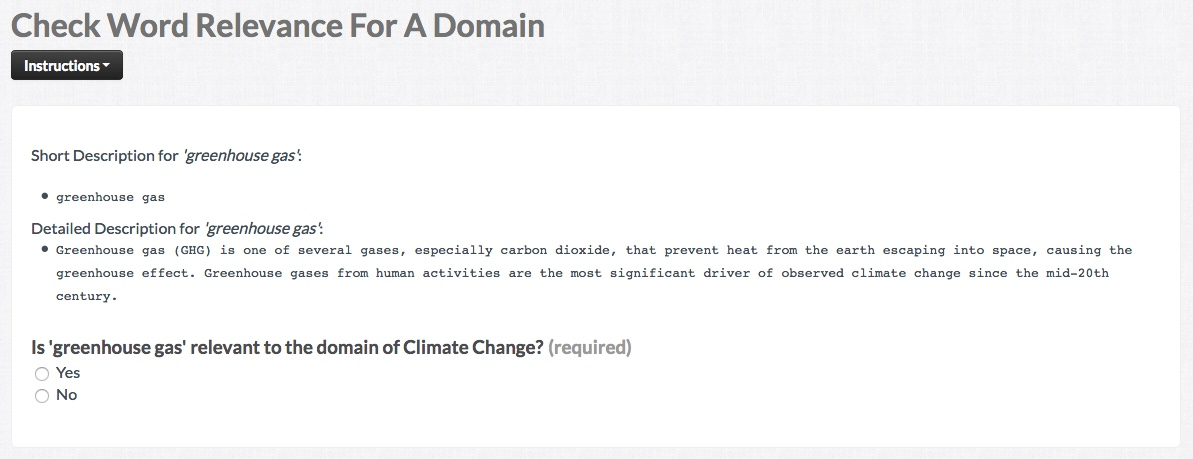
\includegraphics[width=\textwidth]{screenshots/questionaire_embedded_context_enrichment}
        \caption{Metadata based Method}
        \label{fig:crowdsourcing_interface_ec}
    \end{subfigure}
	~\\~\\
    \begin{subfigure}[b]{\textwidth}
        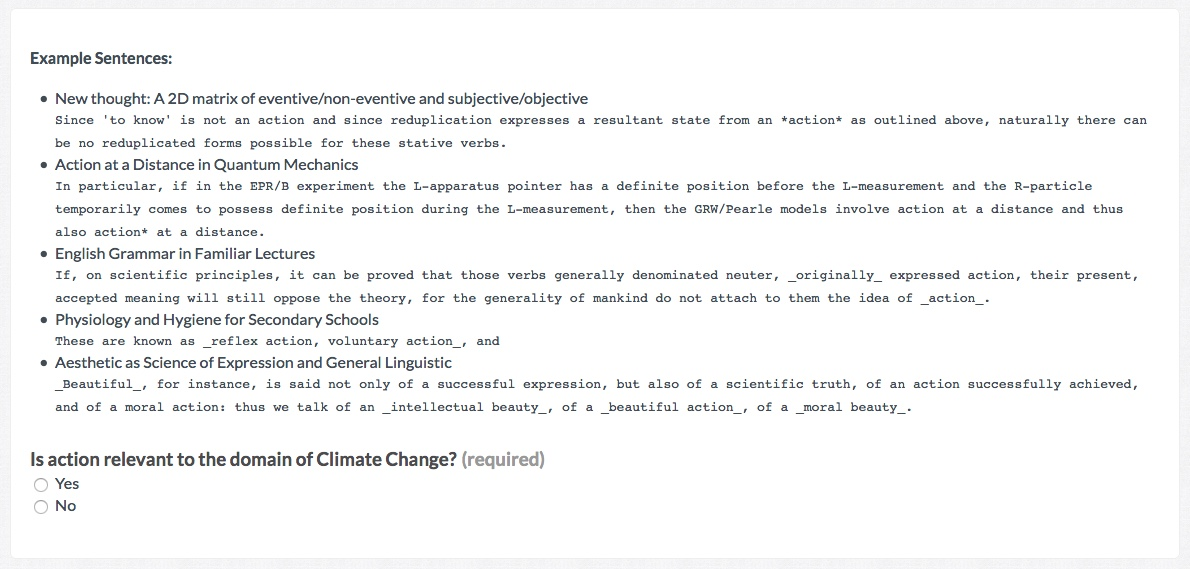
\includegraphics[width=\textwidth]{screenshots/questionaire_wordnik_context_enrichment}
        \caption{Dictionary based Method}
        \label{fig:crowdsourcing_interface_es}
    \end{subfigure}
    \caption{Crowdsourcing task interfaces for performing ontology validation using different methods of Context enrichment}\label{fig:all_crowdsourcing_interfaces}
\end{figure}

Each Crowdsourcing interface consists of
\begin{enumerate}
		\item the Instruction part
		\item the Context part
		\item the Question part
\end{enumerate}

The \emph{Instructions} are very generic and therefore independent of the chosen Context enrichment method. It contains a short description of the task goals and some examples of already answered questions. We did not include the details of ontology validation because first, it would confuse contributors and second, it is not relevant for answering the question. Also, we advised them to browse the Web or contact Wikipedia in case they do not know the answer or are unsure. Furthermore, it encourages contributors to give answers to their best knowledge and improves the overall quality of the collected results.  

The \emph{Context part} is dynamically adjusted based on the chosen approach.
In \hyperref[fig:crowdsourcing_interface_nn]{Figure~\ref*{fig:crowdsourcing_interface_nn}}, the description is generated by the \emph{Ontology based Method}, in which each statement corresponds to a relation. In this example, the concept \emph{fusion} is related by subsumption to 3 other concepts: $ fusion$  \emph{subclassOf} $ \{ heat, action \} $ and $ state $ \emph{subclassOf} $ fusion $. As of now, only subsumption relations are taken into account for the generation of concept descriptions. 
\hyperref[fig:crowdsourcing_interface_ec]{Figure~\ref*{fig:crowdsourcing_interface_ec}} displays the generated description for the concept \emph{greenhouse~gas}. It contains the short description as well as the detailed description.
\hyperref[fig:crowdsourcing_interface_es]{Figure~\ref*{fig:crowdsourcing_interface_es}} shows some example sentences for the concept \emph{action} which were obtained from WordNik. Thereby each sentence is prepended by a headline written in bold letters. Currently, the plugin only supports WordNik as sentence provider. 

The \emph{Question part} contains the actual question. To prevent spamming, we added a minimum time of $10$ seconds to answer the question. Due to the suggestive nature of the questions, contributors can not skip certain questions in case of uncertainty. This ensures completeness of the result set.

